\documentclass[12pt]{article}
\usepackage[T2A]{fontenc}
\usepackage[utf8]{inputenc}
\usepackage[english, russian]{babel}

\usepackage[left=1.5cm,right=1.5cm,
    top=2cm,bottom=2cm,bindingoffset=0cm]{geometry}

\usepackage{hyperref}
\hypersetup{
    colorlinks=true,
    linkcolor=blue,
    filecolor=magenta,      
    urlcolor=cyan,
    pdftitle={Overleaf Example},
    pdfpagemode=FullScreen,
    }

\urlstyle{same}

\usepackage{graphicx}
% \graphicspath{ {./images/} }

\usepackage{wrapfig}
\usepackage[rightcaption]{sidecap}

\begin{document}
\title{Моделирование барьера диффузии инертного газа через клапаннную структуру на торце нанотрубки

Модель нанотрубки (12.0) с клапанной структурой из четырех цианоформных групп на её торце}
\author{А.Ю. Дроздов}
\date{январь 2024}

\begin{titlepage}
\maketitle
\end{titlepage}

Целью данной работы является исследование возможности создания такой молекулярной структуры наномембраны, при которой условия для диффузии молекул (атомов) газа в одном направлении были бы более благоприятными, чем условия для диффузии таких же молекул газа в противоположном направлении.

Ранее идея создания молекулярной структуры, в которой бы осуществлялись неодинаковые условия для теплового движения молекул в противоположных направлениях, излагалась в статье \cite{Drozdov2001}.

Прежде всего, представляется здесь необходимым разъяснить коренное отличие обсуждаемой идеи от классического «Демона максвелла». Классический «Демон Максвелла» предполагал создание устройства молекулярных размеров, которое было бы способно отличать быстро движущиеся молекулы от медленных и сортировать их по разные стороны мембраны. Неосуществимость такого устройства обусловлена рядом причин, на которых нет необходимости подробно останавливаться здесь, ибо они подробно описаны в литературе. Достаточно назвать здесь ту причину, что подобное устройство для отличия быстрых молекул от медленных должно обладать неким миниатюрным «интеллектом», осуществление которого потребовало бы затрат энергии. 

С другой стороны, ряд экспериментаторов пошли по другому пути создания успешно работающих устройств. Этот путь лишь отдалённо напоминает упомянутый классический «демон Максвелла», но на самом деле таковым не является. Успешные экспериментальные работы были осуществлены в направлении создания условий, в разной степени благоприятствующих тепловому движению частиц в противоположных направлениях. 

В работе \cite{Lavrentjev1992} в качестве тепловых частиц использовались электроны, условия для теплового дрейфа которых создавались неравномерным в пространстве, но постоянным во времени магнитным полем. 

%В работе [3] экспериментально показана неодинаковая проводимость тепловых фононов (теплопроводность) через специальный образом  обработанную нанотрубку.

В работе \cite{KanaevMalinovsky1982} была экспериментально показана неодинаковость объёмной проводимости сегнетоэлектрического кристалла вдоль оси поляризации при изменения направления приложенного напряжения на противоположное.

\begin{wrapfigure}{l}{0.6\textwidth}
    \centering
    \includegraphics[scale=0.35]{./nanotube_12_membrane_4_tricyanomethyl/nanotube_membrane_12.0_4cyanoforms_wdv.png}
    \caption{Модель нанотрубки (12.0) с клапанной структурой из четырех цианоформных групп на её торце}
   % \label{fig:frame_center}
\end{wrapfigure}

В данной работе мы собираемся исследовать такие факторы, влияющие на диффузию газа через мембрану, как 1) потенциальный барьер и 2) стерические (пространственные) затруднения.

Методом решения поставленной задачи является численный эксперимент. Для постановки численного эксперимента за основу мною была взята свободно распространяемая в Интернете (free software) программа ghemical-1.90. Лицензия на которую (GNU GPL), предоставляет право изменять её и дальше распространять.

Репозиторий с модифицированной автором программой, использованной в данном моделировании расположен по адресу  \url{https://github.com/daju1/winlibghemical}

Модель нанотрубки (12.0) с клапанной структурой из четырех цианоформных групп на её торце, папка \url{https://github.com/daju1/moldyn/tree/main/nanotube_12_membrane_4_tricyanomethyl_prob_atom/}

Мы меняем координату пробной частицы, и при этом вычисляем как изменяется энергия взаимодействия этой пробной частицы с остальными частицами. И если мы вдавливаем нашу пробную частицу внутрь группы остальных частиц, мы их деформируем. А раз мы их деформировали, значит мы должны дать некоторое время на то, чтобы деформация остальных частиц пришла к своему минимуму потенциальной энергии. При этом остальные частицы меняют свое взаимное расположение. Если мы нашу пробную частицу продавливаем внутрь массы остальных частиц достаточно медленно, то остальные частицы успевают за время продавливания прийти к своему минимуму потенциальной энергии. Такой процесс обычно называют равновесным.

%
%\begin{figure}
%\centering
%\includegraphics{./work_6H_CN_He/5_plots_1001_nstep=500.png}
%\caption{кадр назад, состояние 1}
%\end{figure}

%\begin{wrapfigure}{r}{0.5\textwidth}
%    \centering
%    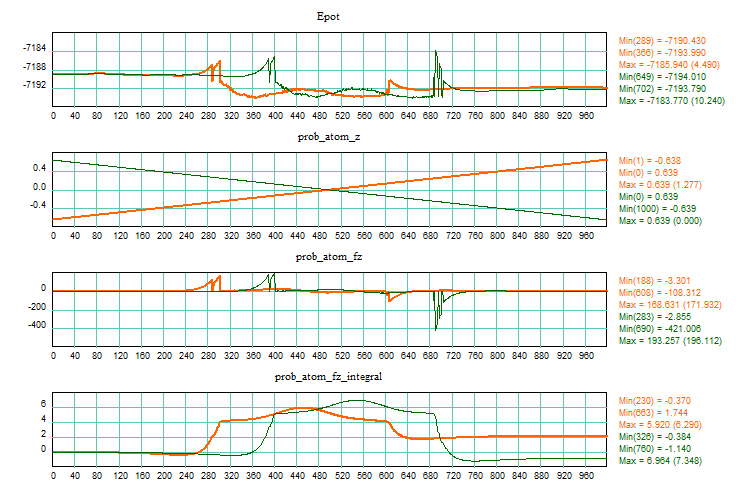
\includegraphics[scale=0.5]{./nanotube_12_membrane_4_tricyanomethyl_prob_atom/4_plots_1001_nstep=500_fix_z.png}
%    \caption{потенциальная энергия деформации мембранной молекулярной системы Epot и работа проталкивания пробного атома сквозь мембрану prob\_atom\_fz\_integral в прямом направлении и в обратном направлении при фиксировании у пробного атома всех трёх координат}
%    \label{fig:frame_center}
%\end{wrapfigure}


\begin{wrapfigure}{R}{0.7\textwidth}
    \centering
    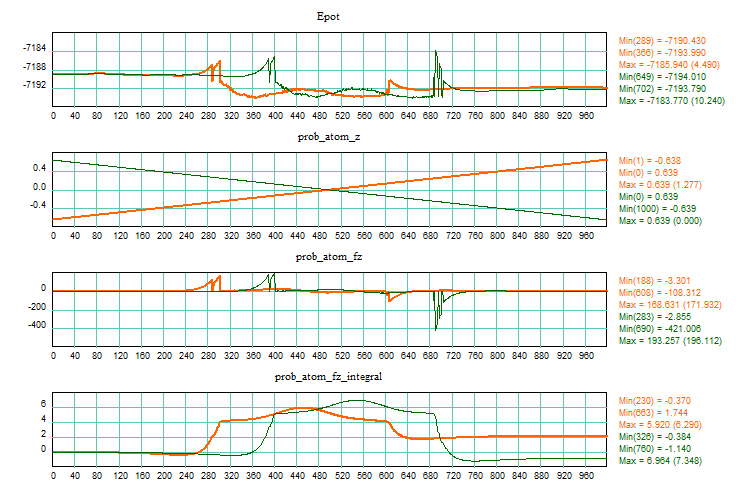
\includegraphics[scale=0.7]{./nanotube_12_membrane_4_tricyanomethyl_prob_atom/4_plots_1001_nstep=500_fix_z.png}
    \caption{потенциальная энергия деформации мембранной молекулярной системы Epot и работа проталкивания пробного атома сквозь мембрану prob\_atom\_fz\_integral в прямом направлении и в обратном направлении при фиксировании у пробного атома z координаты}
    \label{fig:frame_center}
\end{wrapfigure}



Чтобы промоделировать равновесный процесс продавливания пробной частицы нужно задать достаточно большое число итераций в алгоритме оптимизации геометрии. А как работает этот алгоритм? Очень просто. Он вычисляет потенциальную энергию взаимодействия частиц, вычисляет также и градиент этой потенциальной энергии по координате каждой незафиксированной частицы и производит шаг градиентного спуска по этому сложному функционалу потенциальной энергии. В этом алгоритме я могу регулировать критерии остановки этого алгоритма. Самый простой критерий: число итераций. А чему соответствует число итераций градиентного спуска? Приблизительно можно допустить что это число пропорционально времени, которое мы отпускаем на релаксацию деформированной системы частиц.


Для данной молекулярной структуры при выбранном шаге изменения координаты пробного атома для того, чтобы процесс продавливания можно было считать равновесным, достаточно было установить 100 итераций оптимизации геометрии.

Начинаю цикл моделирований 1001 фрейм симуляции с 500 итерациями оптимизации геометрии. То есть режим моделирования максимально приближенный к равновесному.

Используя конфигурацию программы:  фиксируем у пробного атома все три координаты

%\#define PROBNIY\_ATOM\_GEOMOPT 1

%\#define PROBNIY\_ATOM\_FIXED\_AND\_GEOMOPT 1 –

%\#define PROBNIY\_ATOM\_GEOMOPT\_TRADITIONAL 0

%\#define USE\_BOUNDARY\_OPT\_ON\_PROBNIY\_ATOM\_GEOMOPT 0


Поскольку структура клапана не является центральносимметричной, то фиксирование всех трёх координат пробного атома привело, как это видно из характера графика, к часто осциллирующим значениям энергии между различными энергетическими уровнями. 

Следующее моделирование при фиксировании у пробного атома только лишь z координаты показало, что 

потенциальная энергия деформации мембранной молекулярной системы Epot 12.5 кДж/моль в прямом направлении и 19.5 кДж/моль в обратном направлении

работа проталкивания пробного атома сквозь мембрану prob\_atom\_fz\_integral 14.235 кДж/моль в прямом направлении и 23.384 кДж/моль в обратном направлении (при числе итераций оптимизации 500)

В данной молекулярной модели величина барьера по порядку величины соответствует величине средней энергии поступательного движения молекул 1/2*R * T = 0,5 * 8.314 * 300/1000 = 1.247 кДж / моль.


анизотропия по направлению движения пробного атома наблюдается как для потенциальной энергии деформации мембранной молекулярной системы Epot, так и для работы проталкивания пробного атома сквозь мембрану prob\_atom\_fz\_integral. 

Итак, в результате данного исследования можно прийти к выводу о том, что асимметрия, связанная с инверсией направления движения пробной частицы проявляется также и в случае равновесного моделирования, что указывает на возможность реализации синтетического демона Максвелла


\begin{thebibliography}{99}

\bibitem{Drozdov2001}
\textit{ Дроздов А.Ю. Синтетический демон Максвелла. – Химия и жизнь, 2001, № 12, с. 62 – 63. \url{http://daju.narod.ru/Maxwell/SintMaxwDem.pdf} }

\bibitem{Lavrentjev1992}
\textit{ Лаврентьев О.А. Экспериментальное доказательство возможности преобразования тепловой энергии хаотического движения частиц непосредственно в электрическую. – Препринт ХФТИ № 92-24 – Харьков, 1992 – 16 с. \url{http://www.daju.narod.ru/Maxwell/LavrentyevOA.pdf} }

\bibitem{KanaevMalinovsky1982}
\textit{И. Ф. Канаев, В. К. Малиновский, Асимметрия
проводимости вдоль оси поляризации в сегнето-
электрических кристаллах, Докл. АН СССР, 1982,
том 266, номер 6, 1367–1370}

\end{thebibliography}

\end{document}
